\section{Hardware for real-world experiments}
    \subsection{Robots}
        In this section, we will present the robots available for use in the real-world experiments. We have two robotic platforms available for us: Husky and Spot.\\\\
        \bfc{Husky}\\
        Husky is a medium all-terrain robot developed by Clearpath Robotics. It is a four-wheeled robot with a payload capacity of 75 kg. The weight of this robot without the payload is 50 kg, and its maximal speed is $1\:\si{\m\per\s}$. This robot is mainly used outside of urban areas. The photo of the Husky in the configuration we use is shown in figure \ref{fig:husky}.\\
        More information about the Husky platform is available at the Clearpath Robotics website\footnote{\url{https://clearpathrobotics.com/husky-unmanned-ground-vehicle-robot/}}.\\\\
        \bfc{Spot}\\
        The Spot is a medium all-terrain robot developed by Boston Dynamics. It is a four-legged robot with a payload capacity of 14 kg. The weight of this robot without the payload is 33 kg, and its maximal speed is $1.6\:\si{\m\per\s}$. This robot is designed to be mainly used in urban and industrial areas. The photo of the Spot robot with our payload is shown in figure \ref{fig:spot}.\\
        More information is available at the Boston Dynamics website\footnote{\url{https://www.bostondynamics.com/sites/default/files/inline-files/spot-specifications.pdf}}.

        \begin{figure}[H]
            \centering
            \begin{subfigure}[b]{0.495\textwidth}
                \centering
                \includegraphics[width=\textwidth]{images/husky.jpg}
                \caption{The Husky robot configuration.}
                \label{fig:husky}
            \end{subfigure}
            \begin{subfigure}[b]{0.495\textwidth}
                \centering
                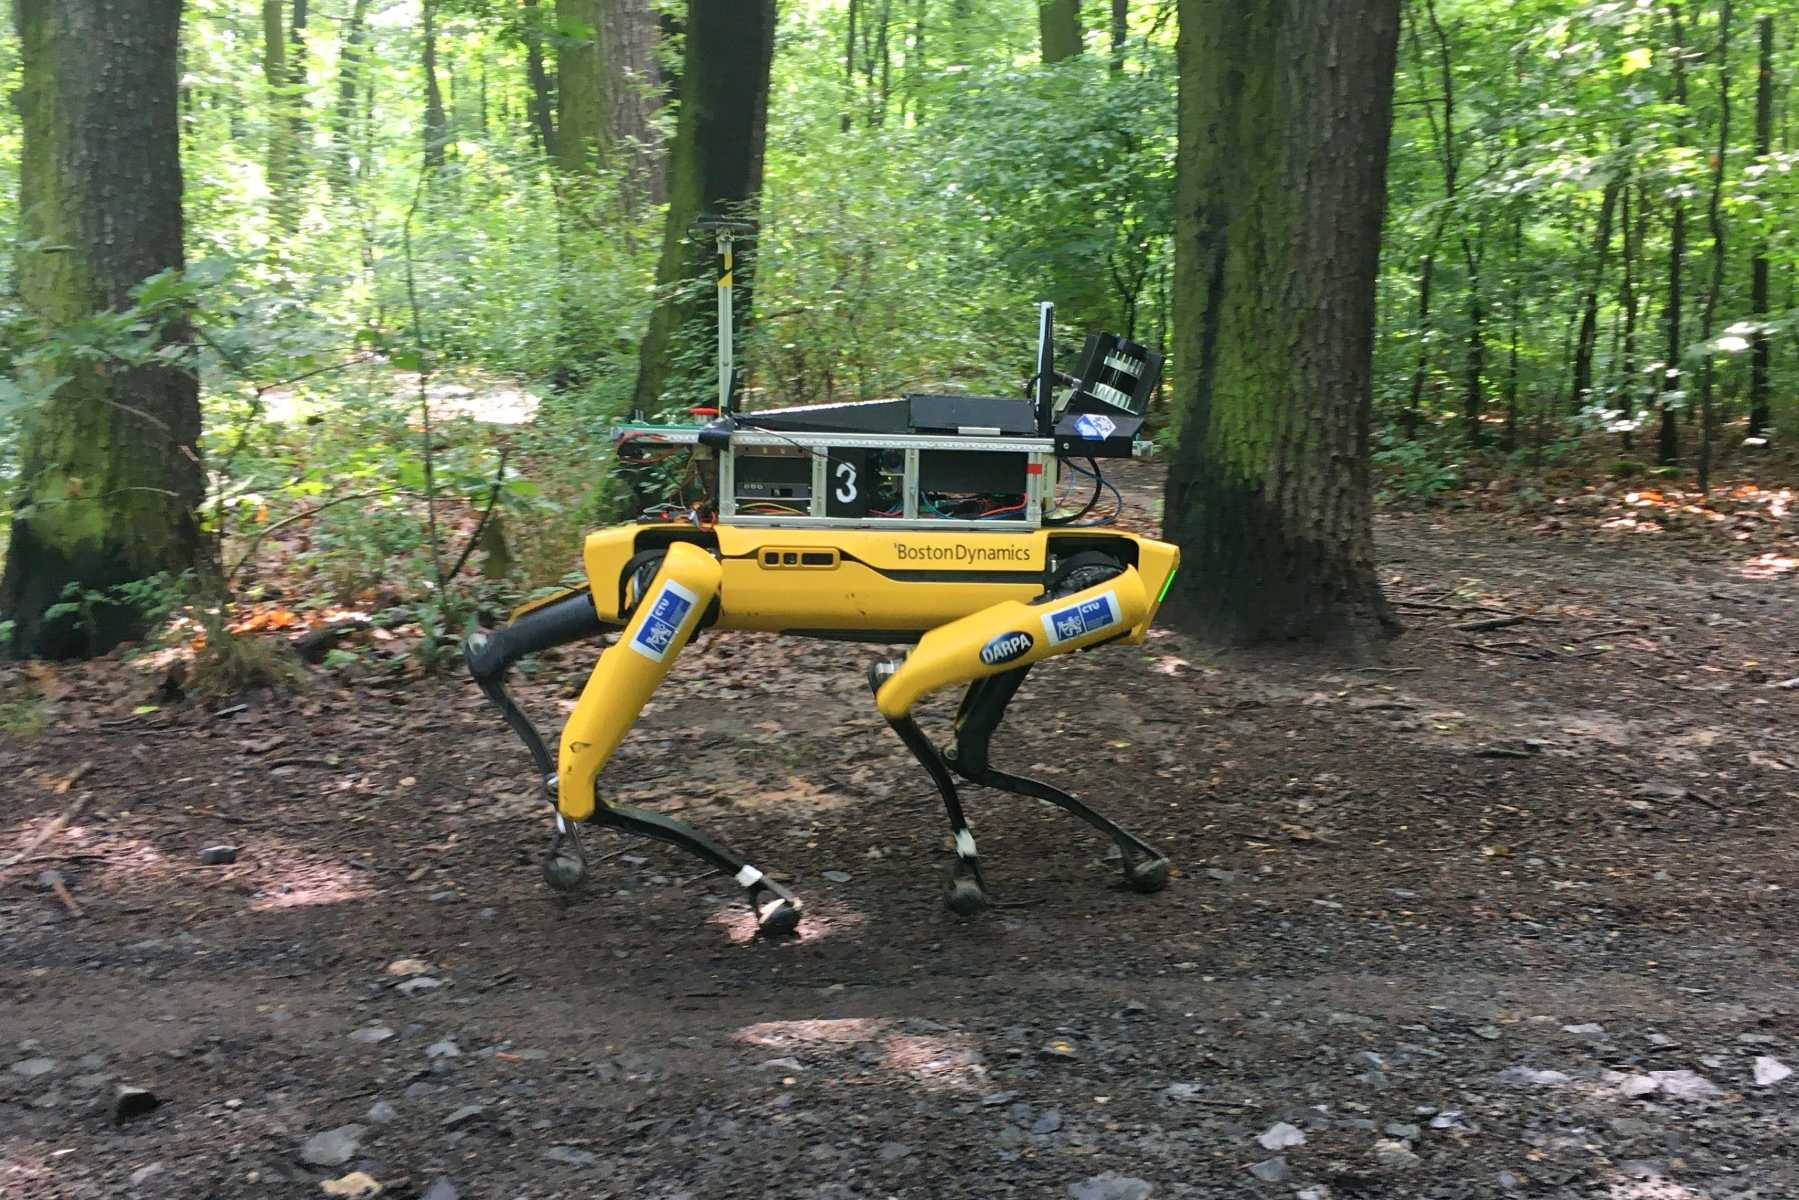
\includegraphics[width=\textwidth]{images/spot.jpg}
                \caption{The Spot robot configuration.}
                \label{fig:spot}
            \end{subfigure}
            \caption{Robots available for real-world experiments.}
        \end{figure}
        \noindent The photos are courtesy of CRAS at FEE CTU.

    \subsection{Sensors}
        The capabilities of our robots are highly dependent on the sensors we attach to them. Without them, the possibilities and options for missions are minimal. In our work, we will use some sensors directly and some indirectly. The indirect usage of sensors is connected with dependencies on other projects. One notable example is the detection of vehicles and other obstacles. This detection is not in the scope of our work but is instrumental to its success. The design of the algorithm was done in a way to not be reliant on a specific sensor for vehicle detection.\\\\
        \bfc{Magnetometer}\\
            This is one of the sensors we use directly. We use it to determine the azimuth of our robot and help it position itself perpendicular to the road it will try to cross.\\
            We say that the sensor is used directly. However, the transformation of the IMU magnetometer data into the azimuth was not implemented as a part of this work.\\\\
        \bfc{Camera}\\
            Our robots are fitted with cameras pointing forward, backward, left, right, and up. This sensor is mostly used to determine the classification of obstacles rather than detecting the obstacles themselves. As this sensor is not vital to the functionality of our algorithm, we will not discuss them further.\\
            The cameras on our robots are GigE Basler ace2 PRO.\\\\
        \bfc{LiDAR}\\
            LiDAR is another essential sensor installed on our robots. It is responsible for detecting approaching vehicles and providing information such as their speed, position vectors, and other relevant parameters. The data generated by LiDAR plays a critical role in our algorithm, as we expect the processed data to serve as the primary condition for determining the velocities during the crossing.\\
            More detailed information on the scanning mechanisms and function of LiDARs can be found in \cite{LiDAR}.\\
            The LiDARs used on our robots are Ouster OS0-128.\\\\
        \bfc{GNSS}\\
            All robots also have a GPS sensor. We use this sensor for precise localization of the robots in the global coordinate system.\\
            The GPS sensors we use are Emlid Reach M+.
